\documentclass[11pt, letterpaper]{article}

% --- 1. Basic Packages (Standard in all LaTeX distributions) ---
\usepackage[utf8]{inputenc}
\usepackage[T1]{fontenc}
\usepackage{amsmath, amssymb, amsthm, amsfonts}
\usepackage{geometry}
\geometry{margin=1in}
\usepackage[hidelinks]{hyperref}

% --- 2. Simplified TikZ (No special libraries to avoid errors) ---
\usepackage{tikz}

% --- 3. Custom Macros (Replacing the physics package to prevent errors) ---
\newcommand{\rs}{r_s}
\newcommand{\dd}{\mathrm{d}}
\newcommand{\pd}[2]{\frac{\partial #1}{\partial #2}}

% --- 4. Metadata ---
\title{\textbf{On the Correspondence Between Schwarzschild Radii and K{\"a}hler-Einstein Metrics}}
\author{Technical Synthesis}
\date{\today}

\begin{document}

\maketitle

\begin{abstract}
This paper investigates the geometric mapping of the Schwarzschild radius ($\rs$) into the complex structure of K{\"a}hler manifolds. The transition from Lorentzian spacetime to Euclidean Riemannian space via Wick rotation is examined.
\end{abstract}

\section{The Schwarzschild Geometry}
The unique vacuum solution to the Einstein field equations for a static, spherically symmetric system is the Schwarzschild metric. The line element is:
\begin{equation}
    ds^2 = -\left(1 - \frac{\rs}{r}\right) dt^2 + \left(1 - \frac{\rs}{r}\right)^{-1} dr^2 + r^2 (d\theta^2 + \sin^2\theta d\phi^2)
\end{equation}
where the Schwarzschild radius $\rs = 2GM$ defines the event horizon. 



\section{Causal Structure}
The event horizon at $r = \rs$ acts as a null boundary. In a conformal representation, this is visualized via a Penrose-Carter diagram.

\begin{figure}[h]
    \centering
    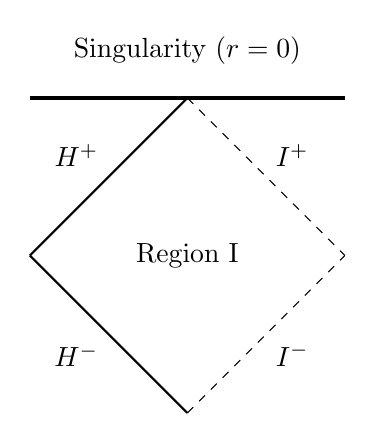
\begin{tikzpicture}[scale=2]
        % Simple Diamond (No complex decorations to avoid "Undefined Control Sequence")
        \draw [thick] (0,0) -- (1,1) node[midway, above left] {$H^+$};
        \draw [thick] (0,0) -- (1,-1) node[midway, below left] {$H^-$};
        \draw [dashed] (1,1) -- (2,0) node[midway, above right] {$I^+$};
        \draw [dashed] (1,-1) -- (2,0) node[midway, below right] {$I^-$};
        
        % Singularity represented as a simple thick double line
        \draw [ultra thick] (0,1) -- (2,1);
        \node at (1,1.3) {Singularity ($r=0$)};
        \node at (1, 0) {Region I};
    \end{tikzpicture}
    \caption{Penrose-Carter diagram of the Schwarzschild spacetime.}
\end{figure}



\section{K{\"a}hler Mapping via Wick Rotation}
To interpret this geometry as a K{\"a}hler manifold, we apply a Wick rotation $t \to i\tau$. This yields the Euclidean Schwarzschild metric. For this geometry to be regular at $r = \rs$, the imaginary time $\tau$ must be periodic:
\begin{equation}
    \tau \sim \tau + 4\pi \rs
\end{equation}



This turns the $(r, \tau)$ plane into the origin of a complex space with a K{\"a}hler structure. On such a manifold, the metric is generated by a K{\"a}hler potential $\mathcal{K}$:
\begin{equation}
    g_{i\bar{j}} = \frac{\partial^2 \mathcal{K}}{\partial z^i \partial \bar{z}^j}
\end{equation}
For a vacuum black hole, the manifold must be Ricci-flat. The Schwarzschild radius $\rs$ dictates the periodicity and boundary conditions of this potential, linking the physical mass scale to the K{\"a}hler-Einstein manifold.

\begin{thebibliography}{99}
\bibitem{Gibbons93} Gibbons, G. W. and Hawking, S. W. (1993). \textit{Euclidean Quantum Gravity}. World Scientific.
\bibitem{Yau78} Yau, S. T. (1978). On the Ricci curvature of a compact K{\"a}hler manifold. \textit{Comm. Pure Appl. Math.} 31, 339.
\end{thebibliography}

\end{document}
